\documentclass{beamer}
\usepackage{grt}

\usetheme{Berlin}
\usecolortheme{seahorse}

\newcommand{\prob}{\mathrm{Prob}}

\title{Reconstructing Phylogenies with Variable Evolution Rates Among Sites}
\author{Garrett Tetrault}
\date{December 5, 2019}

\begin{document}
\frame{\titlepage}

\begin{frame}
    \frametitle{Evolution Rate Model}
    \begin{columns}
        \column{0.6\textwidth}
        \begin{itemize}
            \item We do not assume we know the rate of any given site.
            \item Discrete set of known possible rates $r_i$.
            \item Transition probabilities $P_{ij}$ and 
            equilibrium probabilities $f_i$ assumed to be known.
            \item Each site evolves independently of one another.
        \end{itemize}

        \column{0.52\textwidth}
        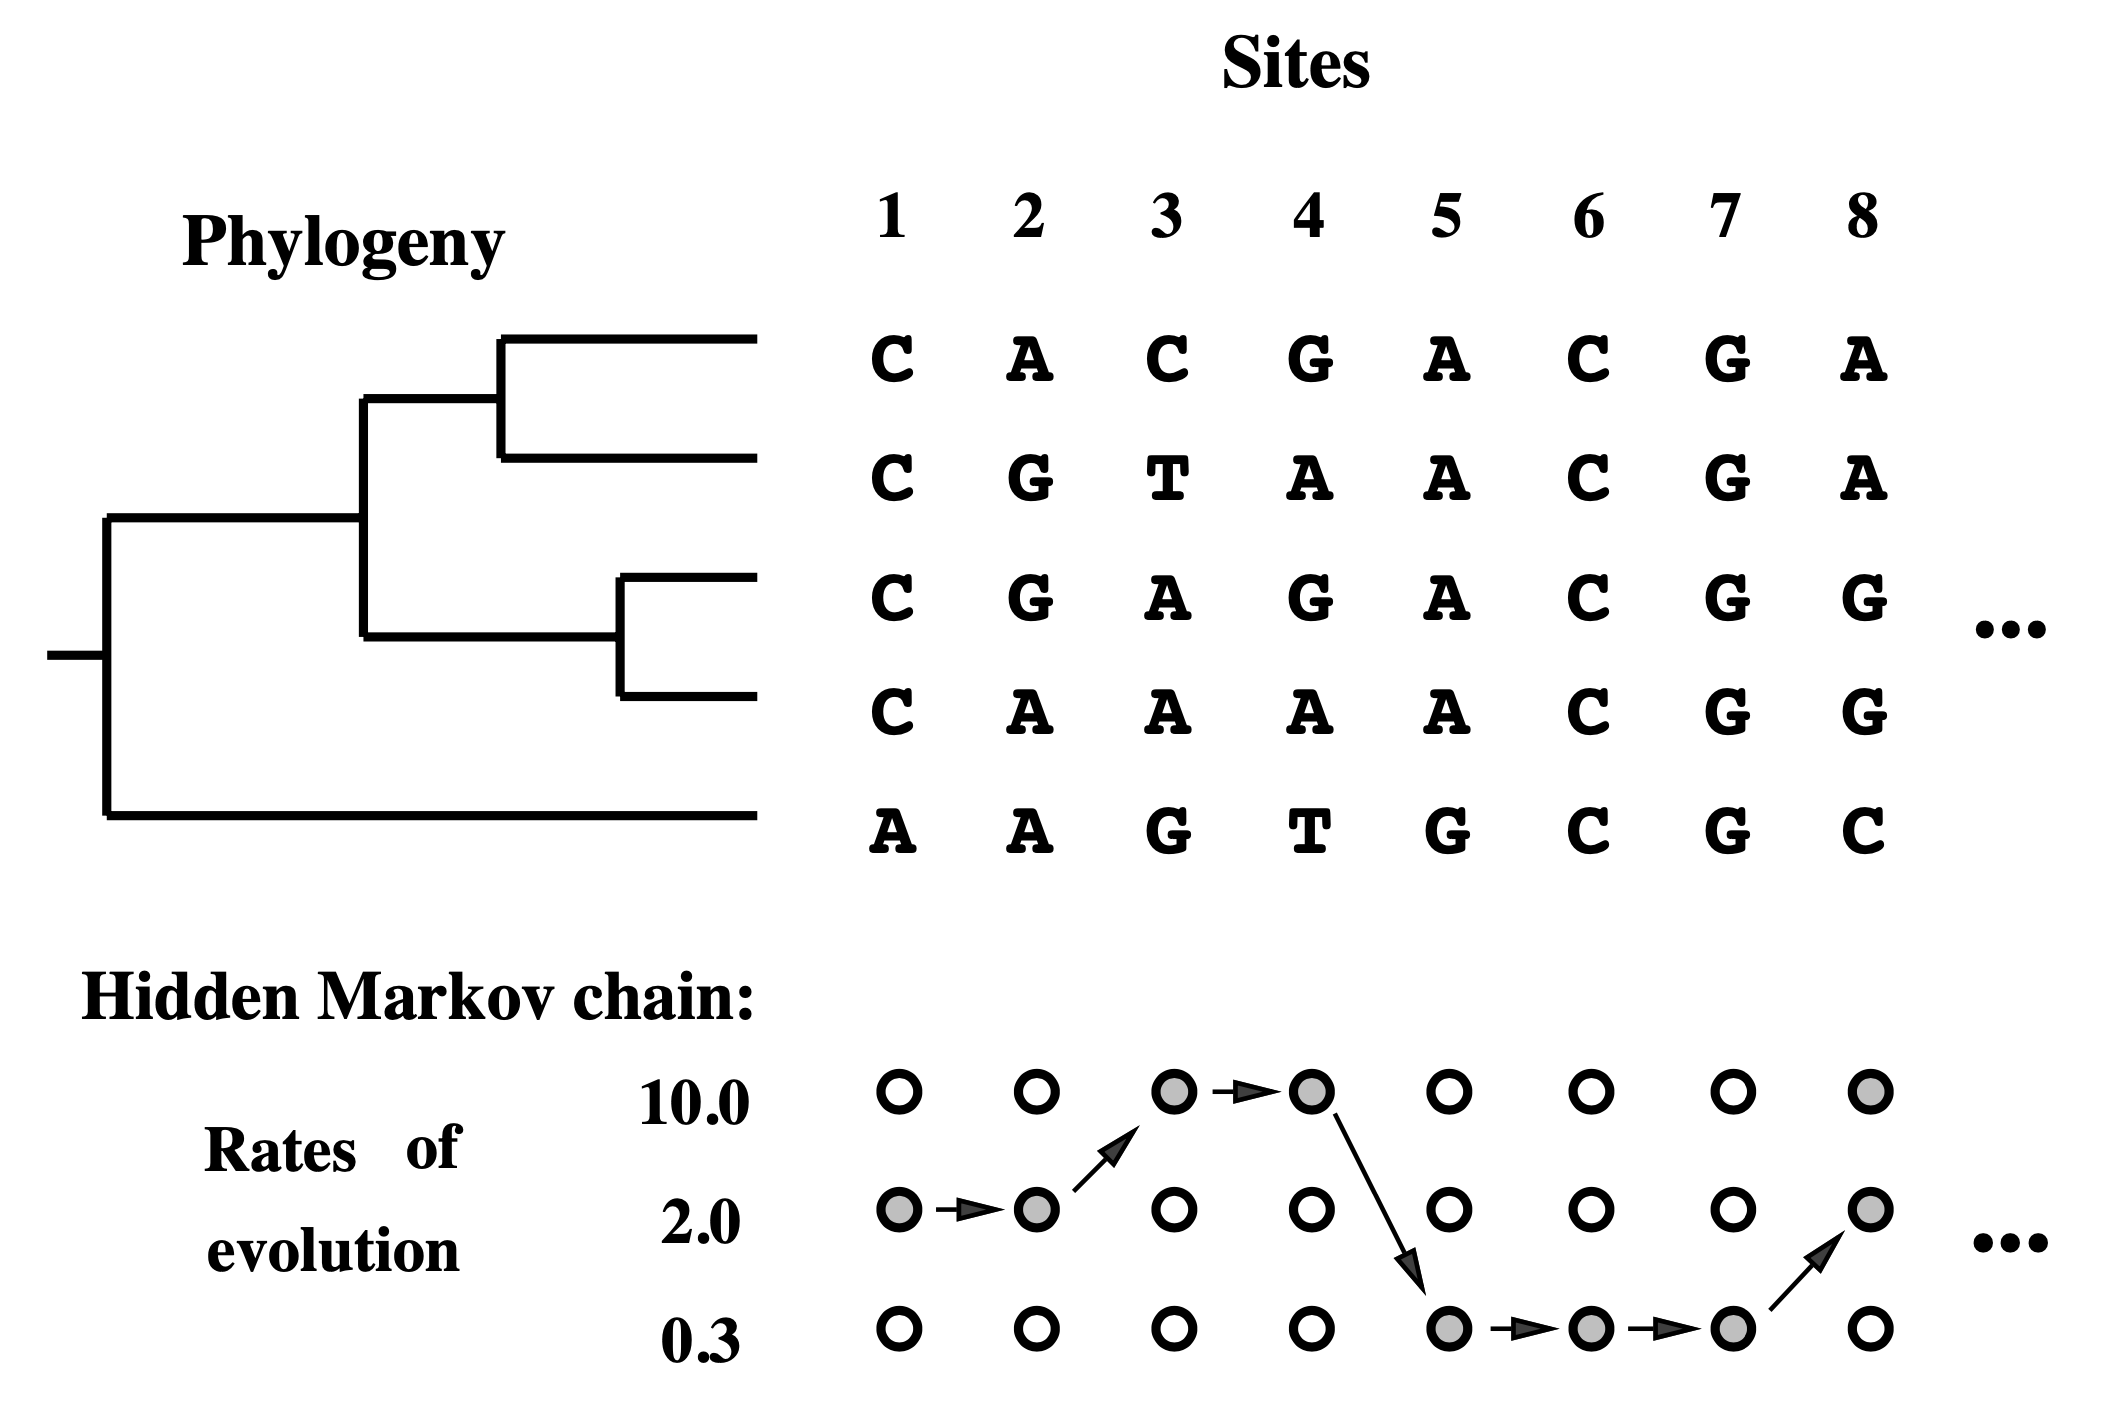
\includegraphics[scale=.15]{hmm_model.png}
    \end{columns}
\end{frame}

\begin{frame}
    \frametitle{Model Likelihood}
    \begin{itemize}
        \item Let $D$ be our data of length $n$ and $T$ a tree topology. 

        \item Likelihood of data 

        \item Let $L$ be the likelihood of the model, 
        and $L_{c_k}^{(k)}$ be the likelihood of $T$ for the data consisting of sites $k$ through $n$
        given that site $k$ has rate category $c_k$.

        \item Then we have,
    \end{itemize}
    \begin{gather*}
        L = \sum_{c_1}f_{c_1}L_{c_1}^{(1)} \\
        L_{c_k}^{(k)} = 
            \prob(D_k \mid T, r_{c_k})
            \sum_{c_{k+1}}P_{c_k, c_{k+1}}f_{c_{k+1}}L_{c_{k+1}}^{(k+1)} \\
        L_{c_n}^{(n)} = 
            \prob(D_n \mid T, r_{c_n})
    \end{gather*}
\end{frame}

\begin{frame}
    \frametitle{Implementation Details}
    \begin{itemize}
    \item We will be using the Jukes-Cantor model of evolution throughout.
    \item Allow branch lengths to be proportional to evolution rate i.e. if $t$ is branch length with evolution rate $r$, we replace $t$ by $rt$.
    \item Simplification of Hasegawa, Kishino and Yano model used in paper.
    \end{itemize}
\end{frame}

\begin{frame}
    \frametitle{Algorithm}
    \begin{itemize}
    \item Tree topologies will be iterated by adding sequences one by one.
    \item Add new sequences by grafting.
        \begin{itemize}
            \item For each potential edge, compute most likely branch length by Newton's method.
        \end{itemize}
    \end{itemize}
    \begin{center}
        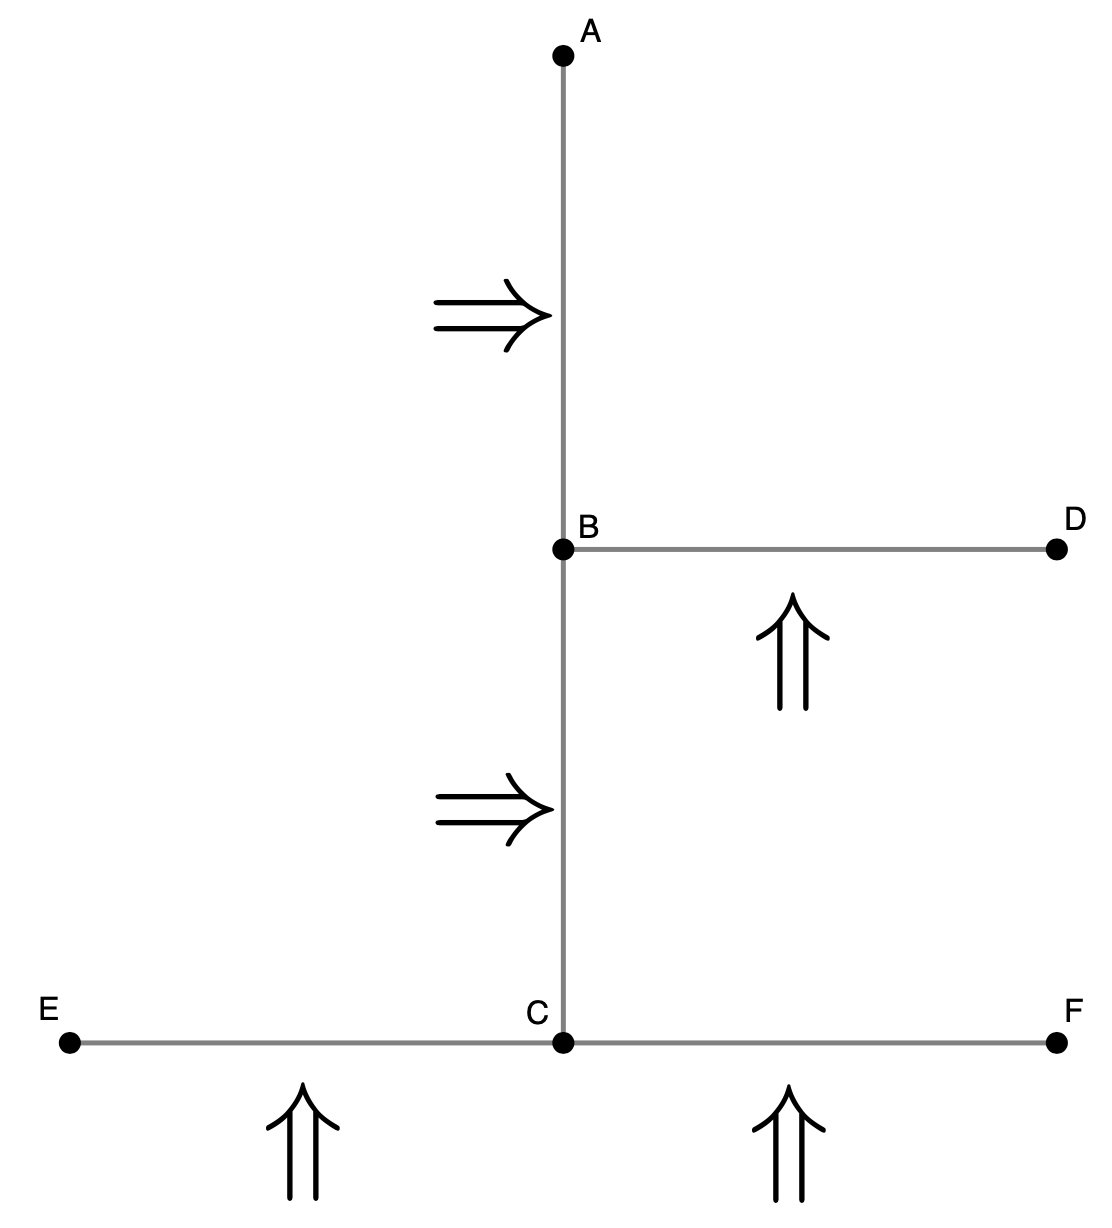
\includegraphics[scale=0.2]{graft.png}
    \end{center}
\end{frame}

\begin{frame}
    \frametitle{Newton's Method}
    \begin{itemize}
        \item Let $(j,k)$ be the new edge we are adding.
        \item Consider likelihood as a function of the branch length $L(v)$.
        \item To maximize, we find $v$ such that $\frac{dL}{dv} = 0$.
        \item Newton's method iterations:
    \end{itemize}
    \begin{gather*}
        v_{i+1} = v_i - \left( \frac{dL}{dv}(v_i) \left/ \frac{d^2L}{dv^2}(v_i) \right. \right)
    \end{gather*}
    \begin{itemize}
        \item Derivatives can be obtained from previous likelihood calculations.
    \end{itemize}
\end{frame}

\begin{frame}
    \frametitle{Calculating Derivatives}
    \begin{itemize}
    \item First derivative:
    \end{itemize}
    \tiny
    \begin{gather*}
        \frac{dL}{dv} = \sum_{c_1}f_{c_1}\frac{dL_{c_1}^{(1)}}{dv} \\
        \frac{dL_{c_k}^{k}}{dv} = 
            \frac{d\prob(D_k \mid T, r_{c_k})}{dv}
            \sum_{c_{k+1}}P_{c_k, c_{k+1}}f_{c_{k+1}}L_{c_{k+1}}^{(k+1)}
            + \prob(D_k \mid T, r_{c_k})
            \sum_{c_{k+1}}P_{c_k, c_{k+1}}f_{c_{k+1}} \frac{dL_{c_{k+1}}^{(k+1)}}{dv} \\
        \frac{dL_{c_n}^{(n)}}{dv} = \frac{d\prob(D_n \mid T, r_{c_n})}{dv}
    \end{gather*}
\end{frame}

\begin{frame}
    \frametitle{Calculating Derivatives}
    \begin{itemize}
    \item Second derivative:
    \end{itemize}
    \tiny
    \[
        \frac{d^2L}{dv^2} = \sum_{c_1}f_{c_1}\frac{d^2L_{c_1}^{(1)}}{dv^2}
    \]
    \begin{align*}
        \frac{d^2L_{c_k}^{k}}{dv^2} 
        =& \left(\frac{d^2\prob(D_k \mid T, r_{c_k})}{dv^2}
            \sum_{c_{k+1}}P_{c_k, c_{k+1}}f_{c_{k+1}}L_{c_{k+1}}^{(k+1)}\right. \\
        &+2\frac{d\prob(D_k \mid T, r_{c_k})}{dv}
            \sum_{c_{k+1}}P_{c_k, c_{k+1}}f_{c_{k+1}}\frac{dL_{c_{k+1}}^{(k+1)}}{dv} \\
        &\left.+\prob(D_k \mid T, r_{c_k})
            \sum_{c_{k+1}}P_{c_k, c_{k+1}}f_{c_{k+1}} \frac{d^2L_{c_{k+1}}^{(k+1)}}{dv^2}\right)
    \end{align*}
    \[
        \frac{d^2L_{c_n}^{(n)}}{dv^2} = \frac{d^2\prob(D_n \mid T, r_{c_n})}{dv^2}
    \]
\end{frame}

\begin{frame}
    \frametitle{Calculating Site-wise Likelihood Derivatives}
    \begin{itemize}
        \item Let $\ell_{ic}^{(m)}(b)$ be the likelihood of $T$ 
        for all data for site $m$ at or above node i on the tree, 
        given that site $m$ in node $i$ is basis $b$, 
        and given that site $m$ has rate category $c$.

        \item Note that this value is computed exactly as in Felsenstein's algorithm.

        \item Let $M_{xy}(t, r) = e^{-\frac{4}{3}tr}\delta_{xy} 
        + \frac{1}{4}\left(1 - e^{-\frac{4}{3}tr}\right)$
        where $\delta_{xy}$ is the Kronecker delta function.
        Note that this is exactly the Jukes-Cantor model.

        \item Then:
    \end{itemize}
    \[
        \prob(D_i \mid T, r_{c_i}) 
        = \frac{1}{4}\sum_x \sum_y \ell_{jc_i}^{(i)}(x) M_{xy}(v, r_{c_i}) \ell_{kc_i}^{(i)}(y)
    \]
\end{frame}

\begin{frame}
    \frametitle{Calculating Site-wise Likelihood Derivatives}
    Equivalently,
    \[
        \prob(D_i \mid T, r_{c_i})
        = e^{-\frac{4}{3}vr_{c_i}}K_1 + K_2
    \]
    where
    \begin{gather*}
        K_1 = \frac{1}{4}\sum_x \sum_y 
            \ell_{jc_i}^{(i)}(x) \left(\delta_{xy} - \frac{1}{4}\right) \ell_{kc_i}^{(i)}(y) \\
        K_2 = \frac{1}{16}\sum_x \sum_y 
            \ell_{jc_i}^{(i)}(x) \ell_{kc_i}^{(i)}(y)
    \end{gather*}
\end{frame}

\begin{frame}
    \frametitle{Calculating Site-wise Likelihood Derivatives}
    From this,
    \begin{gather*}
        \frac{d\prob(D_i \mid T, r_{c_i})}{dv} = -\frac{4}{3}r_{c_i}e^{-\frac{4}{3}vr_{c_i}}K_1 \\
        \frac{d^2\prob(D_i \mid T, r_{c_i})}{dv^2} = \left(\frac{4}{3}r_{c_i}\right)^2e^{-\frac{4}{3}vr_{c_i}}K_1
    \end{gather*}
\end{frame}

\begin{frame}
    \frametitle{Experimentation}
    \begin{itemize}
    \item We can vary both rates and equilibrium probabilities of rates.
    \item For example, we can test differences between uniform and geometrically (truncated) distributed rates.
    \item Or test really high rates of evolution with low probability.
    \item etc.
    \end{itemize}
\end{frame}

\begin{frame}
    \begin{center}
        Thank you!
    \end{center}
\end{frame}

\end{document}